
\documentclass[hyperref={breaklinks=true},fleqn,mathserif]{beamer}
%\documentclass[draft,hyperref={breaklinks=true},fleqn,mathserif]{beamer}

% Spausdinimui ant popieriaus:
%\documentclass[hyperref={breaklinks=true},fleqn,mathserif,handout]{beamer}
%\usepackage{pgfpages}
%\pgfpagesuselayout{4 on 1}[a4paper,landscape,border shrink=5mm]

\usepackage{algorithmic}

%%%%%%%%%%%%%%%%%%%%%%%%%%%%%%%%%%%%%%%%%%%%%%%%%%%%%%%%%%%%%%%%%%%%%%%%%%%%%%%%
% SI units
\usepackage{siunitx}
%\sisetup{detect-all}
%%%%%%%%%%%%%%%%%%%%%%%%%%%%%%%%%%%%%%%%%%%%%%%%%%%%%%%%%%%%%%%%%%%%%%%%%%%%%%%%

%%%%%%%%%%%%%%%%%%%%%%%%%%%%%%%%%%%%%%%%%%%%%%%%%%%%%%%%%%%%%%%%%%%%%%%%%%%%%%%%
\usepackage[utf8x]{inputenc} % atkomentuoti, jei naudojat utf-8 koduotę
\usepackage[L7x]{fontenc}
\usepackage[english,lithuanian]{babel}
%%%%%%%%%%%%%%%%%%%%%%%%%%%%%%%%%%%%%%%%%%%%%%%%%%%%%%%%%%%%%%%%%%%%%%%%%%%%%%%%

\usetheme{Madrid}
%\usecolortheme{beaver}

% Pašalina Navigation Bar
\setbeamertemplate{navigation symbols}{}

\setbeamersize{text margin left=1em,text margin right=1em}

%\setbeamertemplate{footline}[page number]

%\AtBeginSection[]
%{
%\begin{frame}
%    \frametitle{Turinys}
%    \tableofcontents[currentsection]
%\end{frame}
%}

%\AtBeginSubsection[]
%{
%\begin{frame}
%    \frametitle{Outline}
%    \tableofcontents[currentsection,currentsubsection]
%\end{frame}
%}

\title[Mobilioji akcijų kainų stebėjimo sistema]{Mobilioji akcijų kainų stebėjimo sistema}
\subtitle{Kursinis darbas}
\author{Tautvydas Milčiūnas, IT 3 kursas}
\institute{Vilniaus Universitetas, Lietuva \\
	\smallskip Matematikos ir informatikos fakultetas \\
	\smallskip Kompiuterijos katedra
}
\date{{\scriptsize 2017}}

% slide numbering in Beamer class (Warsaw theme), pagal http://tex.stackexchange.com/questions/8179/slide-numbering-in-beamer-class-warsaw-theme
\defbeamertemplate*{footline}{shadow theme}
{%
	\leavevmode%
	\hbox{\begin{beamercolorbox}[wd=.5\paperwidth,ht=2.5ex,dp=1.125ex,leftskip=.3cm plus1fil,rightskip=.3cm]{author in head/foot}%
			\usebeamerfont{author in head/foot}\insertframenumber\,/\,\inserttotalframenumber\hfill\insertshortauthor
		\end{beamercolorbox}%
		\begin{beamercolorbox}[wd=.5\paperwidth,ht=2.5ex,dp=1.125ex,leftskip=.3cm,rightskip=.3cm plus1fil]{title in head/foot}%
			\usebeamerfont{title in head/foot}\insertshorttitle%
		\end{beamercolorbox}}%
		\vskip0pt%
	}
	
	\newcommand*{\urlw}[1]{\href{#1}%
		{\nolinkurl{#1}}}
	
	\newcommand{\St}{\frac{\partial S}{\partial t}}
	\newcommand{\Sx}{\frac{\partial S}{\partial x}}
	\newcommand{\SDxx}{\frac{\partial}{\partial x}\!\left(\!D_S(x)\Sx\right)}
	\newcommand{\Pt}{\frac{\partial P}{\partial t}}
	\newcommand{\Px}{\frac{\partial P}{\partial x}}
	\newcommand{\PDxx}{\frac{\partial}{\partial x}\!\left(\!D_P(x)\Px\right)}
	\newcommand{\xim}{x_{i-\frac12}}
	\newcommand{\xip}{x_{i+\frac12}}
	\newcommand{\NMV}{N\!-\!1}
	
	
\begin{document}
	\frame[plain]{\titlepage}
	
	\begin{frame}
		\frametitle{Darbo tikslas}
		Sukurti automatizuotą akcijų stebėjimo sistemą, kuri gautų akcijų duomenis iš viešai platinamų tarnybų ir atvaizduotų gautus duomenis dvejais būdais: santraukos ir išplėstiniu.
	\end{frame}
	\begin{frame}
		\frametitle{Darbo uždaviniai}
		Išanalizuoti panašias programėles, suprastį jų turinį, dizaino sprendimus ir pagrindines funkcionalumo savybes. Sudaryti teorinį sistemos modelį aprašant pagrindines programėlės dizaino ir funkcionalumo dalis. Aprašyti pasirinktas technologijas bei jų įgyvendinimą kuriant projektą.
	\end{frame}
	\begin{frame}
		\frametitle{Panašių sistemų analizė}
		\begin{table}\centering
			\begin{tabular}{|l|c|c|ll}
				\cline{1-3}
				\textbf{Funckionalumas} & \textbf{„My Stocks} & \textbf{\href{https://play.google.com/store/apps/details?id=org.dayup.stocks}{„Stocks Realtime}} &  \\
				& \textbf{ Portfolio“}&\textbf{Stock Quotes“}  \\ \cline{1-3}
				Registracija&-&+& \\ \cline{1-3}
				Akcijų rinkos&-&+& \\ \cline{1-3}
				Aplanko kūrimas&+&+& \\ \cline{1-3}
				Akcijų naujinimas&-&+& \\ \cline{1-3}
				Akcijų pirkimas&+&+& \\ \cline{1-3}
				Valiutų keitimas&-&-& \\ \cline{1-3}
			\end{tabular}
		\end{table}
	\end{frame}
	\begin{frame}
		\frametitle{Funkciniai sistemos reikalavimai}
		\begin{enumerate}
			\item Turi būti įgyvendintas vartotojo portfelio langas.
			\item Turi būti įgyvendintas akcijų duomenų gavimas iš išorinių šaltinių.
			\item Turi būti įgyvendintas grafikų atvaizdavimas ir keitimas.
			\item Turi būti įgyvendintas valiutų keitimo langas.
		\end{enumerate}
	\end{frame}
	\begin{frame}
		\frametitle{Naudotos technologijos}
		\begin{enumerate}
			\item Expo SDK
			\item React Native
			\item Redux
			\item Genymotion
			\item Yahoo Finance, Quandl ir Highcharts (kaip duomenų šaltiniai).
		\end{enumerate}
	\end{frame}
	\begin{frame}
		\frametitle{Programėlės įgyvendinimas}
		\begin{columns}
			\begin{column}{.48\textwidth}
				\begin{block}{Pagrindinis langas}
					% Your image included here
					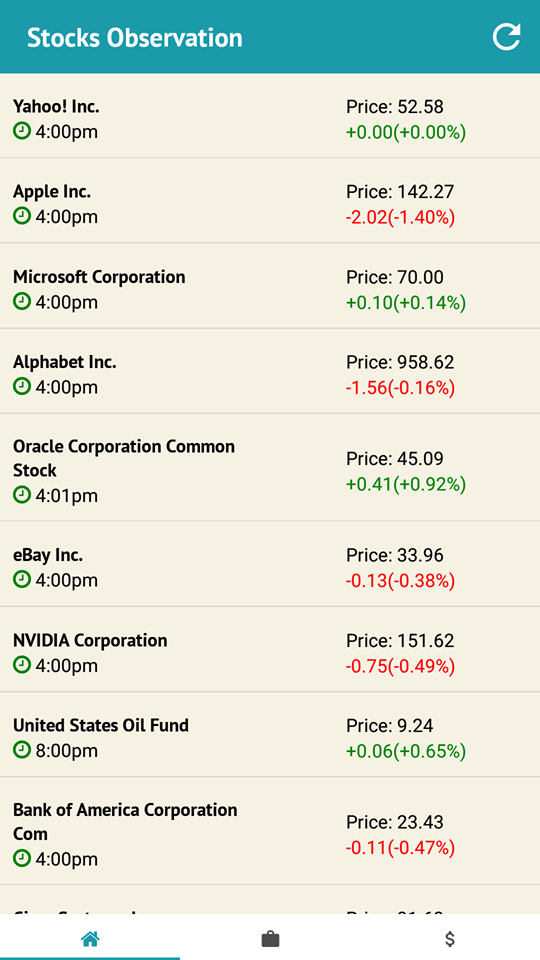
\includegraphics[width=0.65\textwidth]{Pav/home.png}\centering
				\end{block}
			\end{column}
			\begin{column}{.48\textwidth}
				\begin{block}{Grafiko langas}
					% Your image included here
					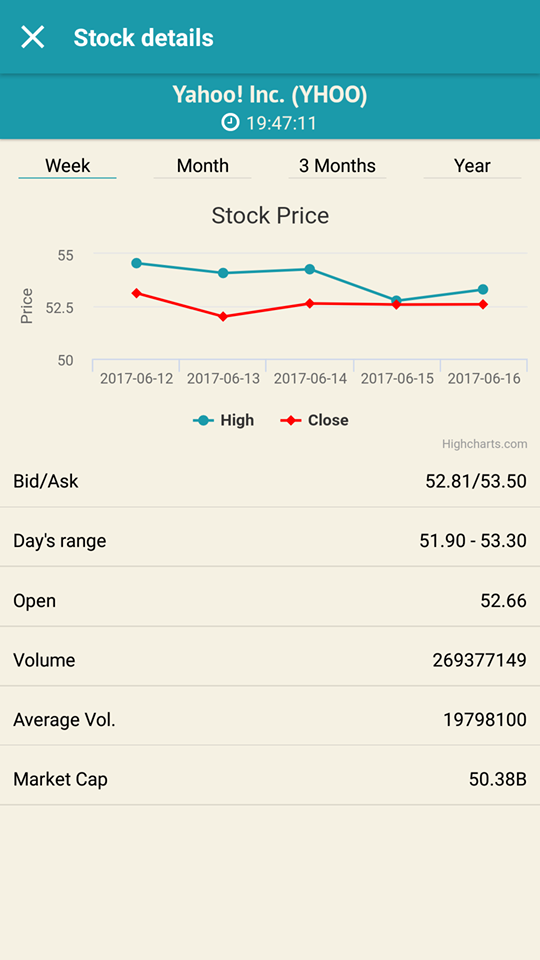
\includegraphics[width=0.65\textwidth]{Pav/stockDetails.png}\centering
				\end{block}
			\end{column}
		\end{columns}
	\end{frame}
	\begin{frame}
		\frametitle{Programėlės įgyvendinimas}
		\begin{columns}
			\begin{column}{.48\textwidth}
				\begin{block}{Vartotojo portfelio langas}
					% Your image included here
					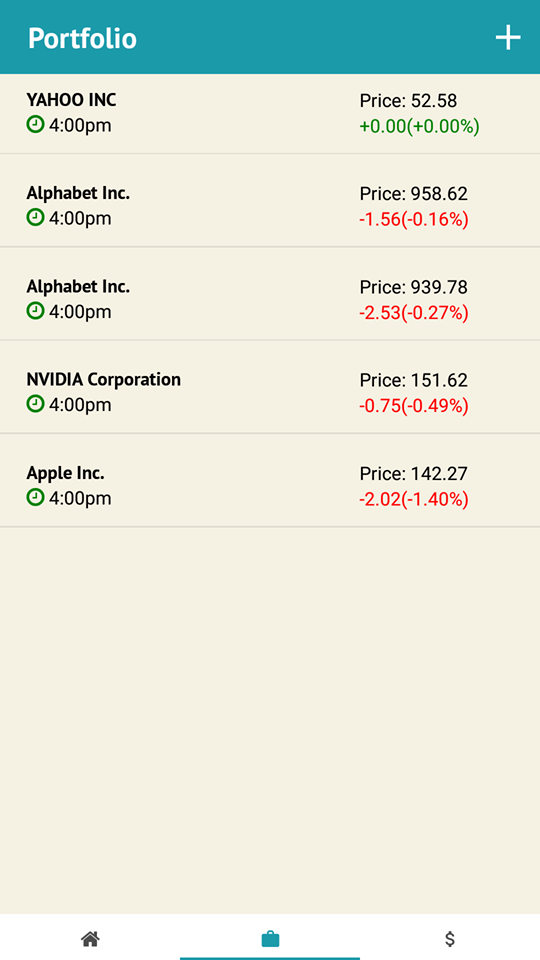
\includegraphics[width=0.65\textwidth]{Pav/portfolio.png}\centering
				\end{block}
			\end{column}
			\begin{column}{.48\textwidth}
				\begin{block}{Paieškos funckionalumas}
					% Your image included here
					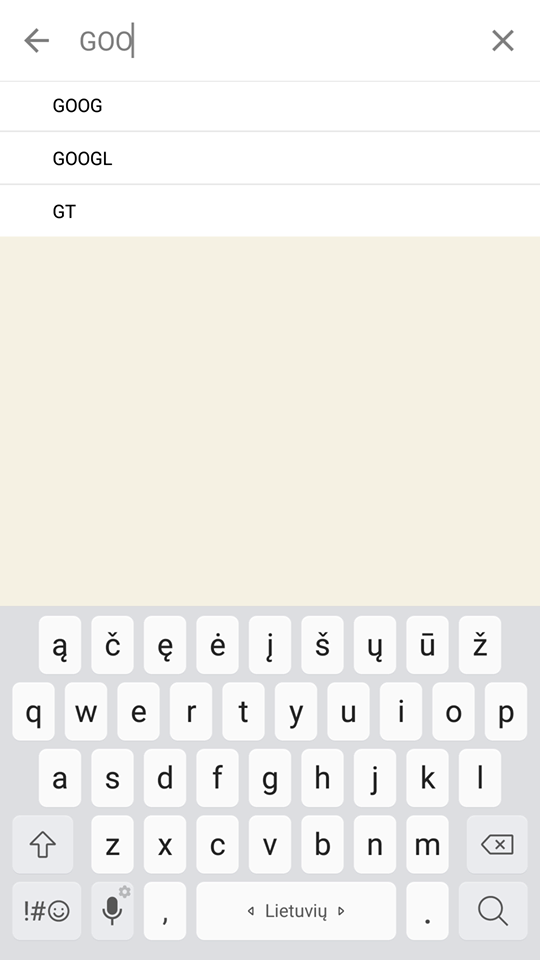
\includegraphics[width=0.65\textwidth]{Pav/stockSearch.png}\centering
				\end{block}
			\end{column}
		\end{columns}
	\end{frame}
	\begin{frame}
		\frametitle{Programėlės įgyvendinimas}
		\begin{columns}
			\begin{column}{.48\textwidth}
				\begin{block}{Valiutų keitimo langas}
					% Your image included here
					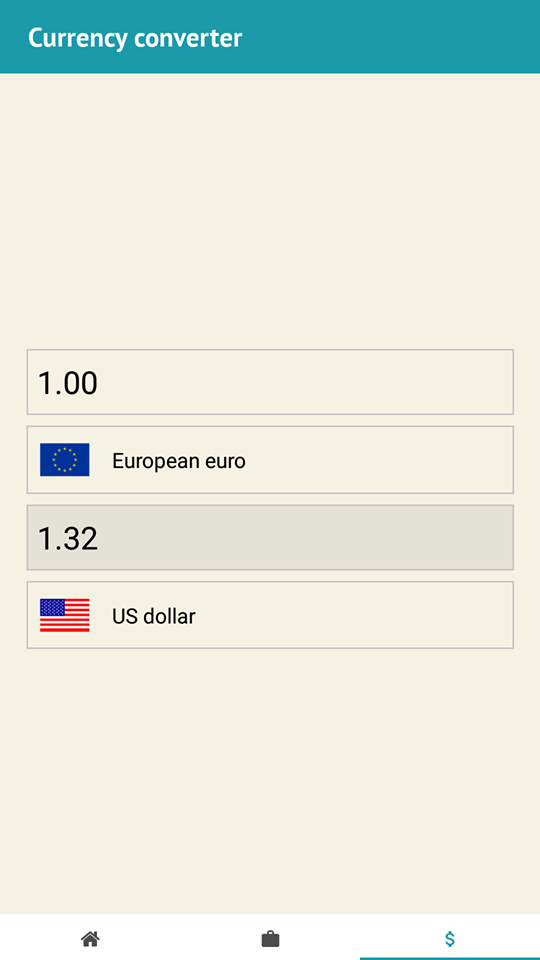
\includegraphics[width=0.65\textwidth]{Pav/currency.png}\centering
				\end{block}
			\end{column}
			\begin{column}{.48\textwidth}
				\begin{block}{Valiutos pasirinkimas}
					% Your image included here
					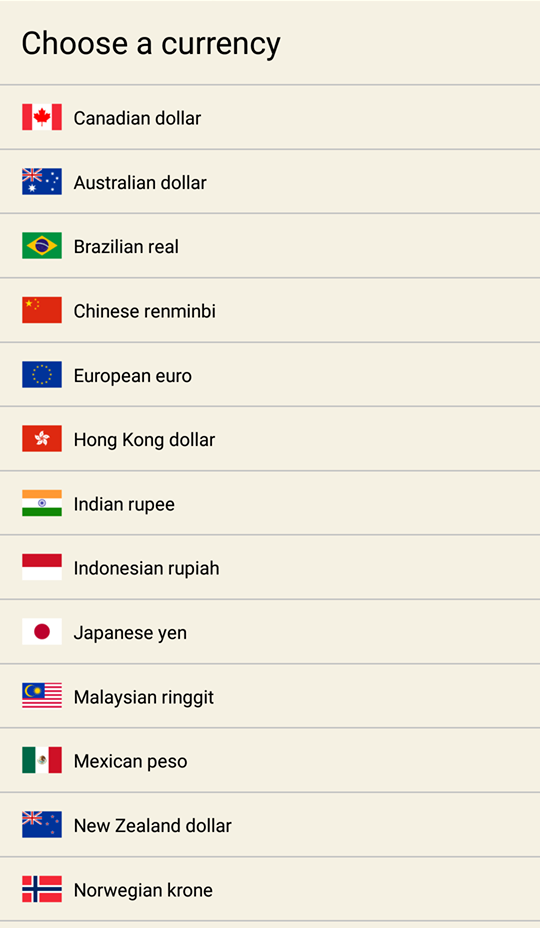
\includegraphics[width=0.65\textwidth, height=0.733\textheight]{Pav/currencySelect.png}\centering
				\end{block}
			\end{column}
		\end{columns}
	\end{frame}
	\begin{frame}
		\frametitle{Išvados}
		\begin{itemize}
			\item Išanalizuotos tokio pat tipo programėlės.
			\item Išanalizuotos ir pritaikytos technologijos skirtos programėlės įgyvendinimui.
			\item Sukurta automatizuota akcijų stebėjimo sistema, kuri atvaizduoja duomenis pagrindiniame ir vartotojo portfelio languose.
		\end{itemize}
	\end{frame}
\end{document}